\section{Működés felvázolása}

Az alkalmazás két \verb=koa= alkalmazásból, számos apró feldolgozó folyamatból,
és a közöttük üzeneteket továbbító üzenetsorból áll (\emph{queue}),
illetve a külvilág egy \emph{reverse proxy}-n keresztül tud ezekhez hozzáférni.


\begin{itemize}
  \item Egy \verb=koa= alkalmazás bonyolítja le a felhasználóval történő
    kommunikációt (\emph{frontend}).
  \item Egy másik \verb=koa= szerver biztosítja az adatbázishoz a hálózaton
    keresztül történő hozzáférést (\emph{db}).
\end{itemize}

Az egyes alkalmazások, és a köztük lévő kapcsolatok \aref{fig:arch}.
ábrán láthatóak. A komponensek függetlenek az őket futtató környezettől,
így tetszőleges számú (fizikai vagy virtuális) hoszton futtathatóak.

\begin{figure}[h!]
  \centering
  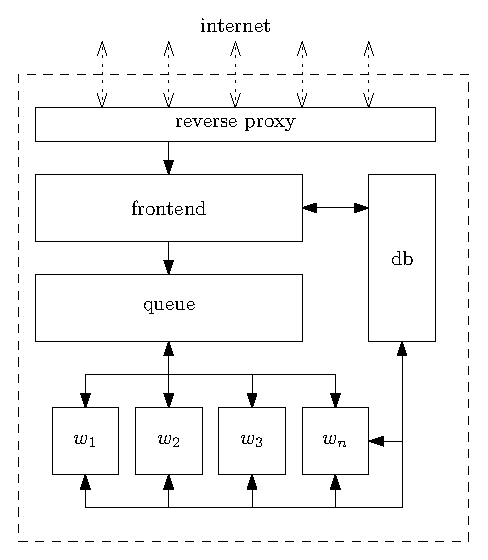
\includegraphics[width=0.6\textwidth]{figures/arch}
  \caption{Az alkalmazás architektúrája}
  \label{fig:arch}
\end{figure}
